\documentclass[../Main.tex]{subfiles}

\begin{document}
\author{Power} %use author for title of lesson
\date{Year 1 Topic 14} %use date to refer to topic in main booklet

\section{Power} %Section is the title of the lesson repeated, ready for the main contents page.

\begin{frame}{Definitions}
    \begin{block}{Can you recall the definition for power from GCSE?}
        \pause 
        Power is the rate of transfer of energy. Or the work done per unit time. 
    \end{block}
    \pause
    \begin{block}{Now, recall our definition of the Volt:}
       \pause 
       1 Volt is defined as 1 Joule of work being carried out on 1 Coulomb of charge.
    \end{block}

\end{frame}

\begin{frame}{Power}
    \begin{equation*}
        P=\frac{\Delta W}{\Delta t} \mbox{and } V=\frac{W}{Q}
    \end{equation*}
    By substitution,
    \begin{equation*}
        P=\frac{V\Delta Q}{\Delta t}
    \end{equation*}
    Yet we know
    \begin{equation*}
        I=\frac{\Delta Q}{\Delta t}
    \end{equation*}
    Hence,
    \begin{equation*}
        P=IV
    \end{equation*}
\end{frame}

\begin{frame}{Power}
    There are 2 other equations of power that we can derive using V=IR.
    
    \begin{equation*}
        P=IV
    \end{equation*}
    
    \begin{exampleblock}{Use your mini whiteboard}
    to derive the other power equations
    \end{exampleblock}
    
    \pause
    
    {\huge
    \begin{equation*}
        P=I^2R, P=\frac{V^2}{R}
    \end{equation*}
    }
\end{frame}

\begin{frame}{Examples}
    \begin{exampleblock}{Example 1}
    Calculate the rate of energy transfer of a 3V bulb with an operating current of 0.5A. \pause
    --1.5W
    \end{exampleblock}
    \pause
    \begin{exampleblock}{Example 2}
    Calculate the total energy transferred in a mains-powered kettle with a current of 13A, as it boils in 2 minutes. \pause
    --360kJ
    \end{exampleblock}
    \pause
    \begin{exampleblock}{Example 3}
    Calculate the rate of energy transfer of a mains toaster with an electrical resistance of 24$\Omega$. Hence, determine the total energy transferred during the 5 minutes it takes to toast. \pause
    -- 2200W, 660kJ
    \end{exampleblock}
    \pause
    --your turn! Have a go at the Kerboodle textbook questions on page 160.
\end{frame}

\begin{frame}{The kilowatt-hour}
    In terms of electrical energy usage, we can think of more practical units than Joules. It is typically better to think in more day-to-day terms. \newline
    
    Most electrical appliances have a power rating -- e.g. a computer may have a power supply of upwards of 1000W (1kW) or higher! We know power $\times$ time is energy used, so if we use an amount of power in an hour we obtain a more reasonable kilowatt-hour as a unit. \newline
    
    This is much easier to picture than the equivalent amount of Joules --
    \begin{exampleblock}{Convert}
    Convert 1kWh to Joules. \pause
    --3.6 MJ!
    \end{exampleblock}
\end{frame}

\begin{frame}{It's about power}
    \begin{figure}
        \centering
        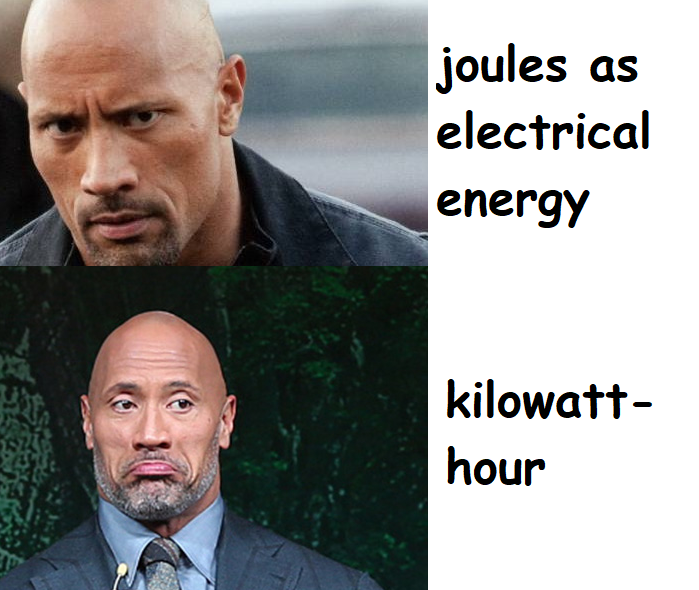
\includegraphics[height=7cm]{Electricity_Images/its_about_power.png}
    \end{figure}
\end{frame}

\begin{frame}{Paying for Electricity}
    As you may (or may not) know -- electricity comes at a price. It is not free, and we, the consumer, must pay for it. \newline
    
    To do so, we typically pay a rate in terms of pence per kilowatt-hour - the current energy price cap is around 25 p/kWh\footnote{An exam question would tell you the cost to use}. In terms of the bill, the cost is the rate multiplied by how many kWh is used (also referred to as units).
    
    \begin{equation*}
            \mathsterling = rate \times units
    \end{equation*}
    
    \begin{exampleblock}{Example}
     [\emph{student name}] plays on [\emph{his/her/their}] [PlayStation/Xbox], which has a power rating of 200W, and [\emph{he/she/they}] use it for at least [number] hours a day over a weekend, estimate [\emph{his/her/their}] contribution to the yearly household bill if the cost of 1 unit is 25p.
    \end{exampleblock}
    \pause
    Now you try - Kerboodle page 162.
\end{frame}

\begin{frame}{Power loss of a battery}
    Recall last lesson we looked at the internal resistance of a battery. Can you remember the equation? \pause
    
    \begin{equation*}
        \varepsilon = Ir + IR
    \end{equation*}
    \pause
    We can look at the total power supplied by a battery by multiplying each term by I (as P=IV, and `$\varepsilon$', `Ir' and `IR' are all voltages). 
    
    \begin{equation*}
        P_{battery} = P_{loss} + P_{supplied}
    \end{equation*}
    \begin{equation*}
        \varepsilon I = I^2r + I^2 R
    \end{equation*}
    
    Based on this, how could we limit the power loss due to internal resistance? \pause 
    -- simply reduce the internal resistance of the battery! This is why we want our phone batteries to have a low internal resistance - we don't want to waste the energy stored in the battery.
\end{frame}

\begin{frame}{Where does the energy go?}
    In an electrical circuit, we say the power used in a component is the rate of energy usage in it. For a phone battery, energy is wasted overcoming the internal resistance. \newline \newline
    
    But where might that energy go? 
    
    \pause
    
    The energy is wasted as heat - touch an electrical component or battery and you will feel that it might be getting hot. Leave your phone on charge or use it for a prolonged period of time and you will feel it get hot.
\end{frame}

\begin{frame}{Efficiency}
    Which of these would represent a battery with a low internal resistance? Which one is more efficient?
    \begin{figure}
        \centering
        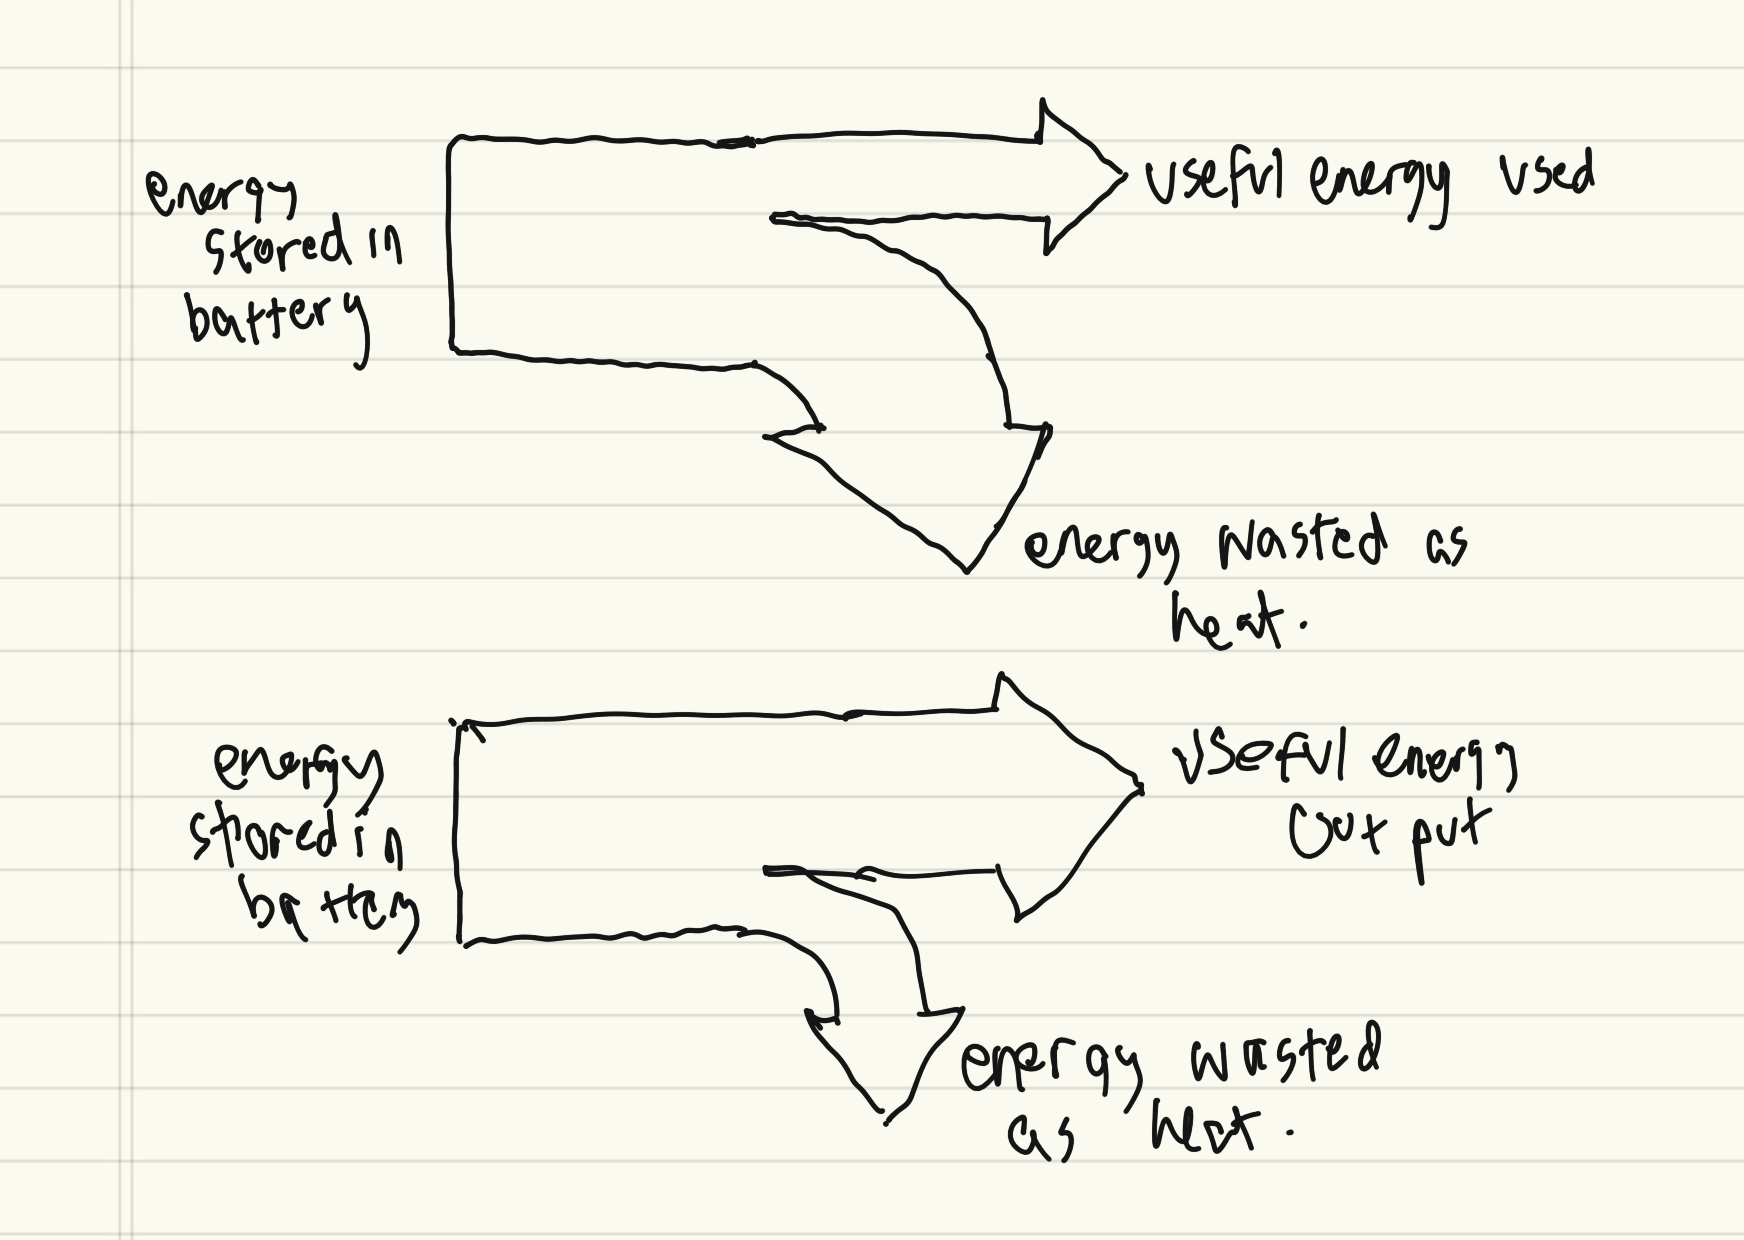
\includegraphics[height=4cm]{Electricity_Images/sankey_diagram.png}
    \end{figure}
    \pause
    \begin{equation*}
        \text{Efficiency} = \frac{\text{useful energy output}}{\text{total energy input}} \times 100\%
    \end{equation*}
\end{frame}

\end{document}